\chapter{Eksperymenty}
% plan eksperymentow, opis danych, wyniki i wnioski
W niniejszym rozdziale przedstawione są eksperymenty, które zostały
przeprowadzone na zebranych wcześniej danych.
Opisany jest sposób ich wykonania, ich wyniki i wnioski, które z nich wynikają.
Na początku w sekcji \ref{section:opisdanych} opisana jest charakterystyka
zebranych danych, a następnie opisuję eksperymenty związane z analizą sentymentu
\ref{section:analizasentymentu2}, analizą geolokacji
\ref{section:analizageograficzna} i analizą grup \ref{section:analizagrup}.


%%%%%%%%%%%%%%%%%%%%%%%%%%%%%%%%%%%%%%%%%%%%%%%%%%%%%%%%%%%%%%%%%%% OPIS DANYCH
\section{Opis zebranych danych}
\label{section:opisdanych}
% 300 slow kluczowych, 18 druzyn, 50 meczow, daty,
% 7 mln tweetów, z tego 300 bylo retweetow, 800 z geolokacja, 
% 900 nijakich

Pomiędzy październikiem a grudniem 2013 roku zebrano 7 263 523 tweety związane
z piłką nożną. Pierwszy z nich ma datę 23 października 15:35:24 a ostatni
29 grudnia 19:27:27. Wszystkie wpisy są powiązane z rozegranymi w tym czasie
35 spotkaniami klubów Arsenal F.C. , Chelsea F.C., Manchester United F.C. i
Manchester City F.C. Daje to średnio 207 529 tweetów na mecz i niecałe
1 815 880 tweetów na drużynę.

Do zbierania tweetów użyte zostały dane 30 drużyn z 538 piłkarzami.
Dodając do tego popularne określenia menadżerów, piłkarzy czy klubów sumarycznie
zebrano 777 słów kluczowych, co daje średnio 22 słowa kluczowe na mecz.

Wpisy zostały stworzone przez 1 567 435 użytkowników, czyli 4.6 
wpisu na użytkownika. 222 545 wpisów zawiera informacje o geolokacji, co stanowi
zaledwie 3.06\% liczby wszystkich wpisów. 666 199 wpisów to odpowiedzi 
(ang. \textit{replies}), to jest 9.17\%, natomiast aż 3 143 060 tweetów
jest retweetami pokrywając 43.27\% danych.

Na tych danych zostały przeprowadzone analizy zaprezentowane w kolejnych podrozdziałach.



% %%%%%%%%%%%%%%%%%%%%%%%%%%%%%%%%%%%%%%%%%%%%%%%%%%%%%%%%%%% ANALIZA SENTYMENTU
\section{Analiza sentymentu}
\label{section:analizasentymentu2}
% 40\% bylo pozytywnych, 30\% negatywnych w meczach Arsenalu byl taki sentyment
% w chelsea sraki
\subsection{Wprowadzenie}
Analiza sentymentu została przeprowadzona zgodnie z algorytmem przedstawionym w
rozdziale \ref{section:analizasentymentu}. W związku z tym, że wpisy typu
retweet nie mogą posiadać sentymentu wszystkie zaprezentowane poniżej analizy
odnoszą się do grupy wpisów nie będących retweetami. To daje nam 4 120 463
tweety, nad którymi były prowadzone badania. W tej grupie 2 005 934 wpisy zostały
oznaczone jako pozytywne -- 48.68\%, a 1 944 448 jako negatywne -- 47,19\%.

\subsection{Sentyment w meczach}
Jak można się spodziewać sentyment w kolejnych spotkaniach jest adekwatny do
osiąganego przez klub wyniku. Gdy drużyna odnosi zwycięstwo wpisy są bardziej
pozytywne, a gdy przegrywa są bardziej negatywne. Poniżej prezentuję wykresy
sentymentu w kolejnych meczach -- sentyment jest liczony jako stosunek liczby
wpisów pozytywnych do sumy wpisów pozytywnych i negatywnych. Wykresy prezentują
kolejne spotkania Arsenalu \ref{image:pozytywnosc-arsenal} oraz Manchesteru
Untied \ref{image:pozytywnosc-munited}.

\begin{figure}[ht!]
\centering
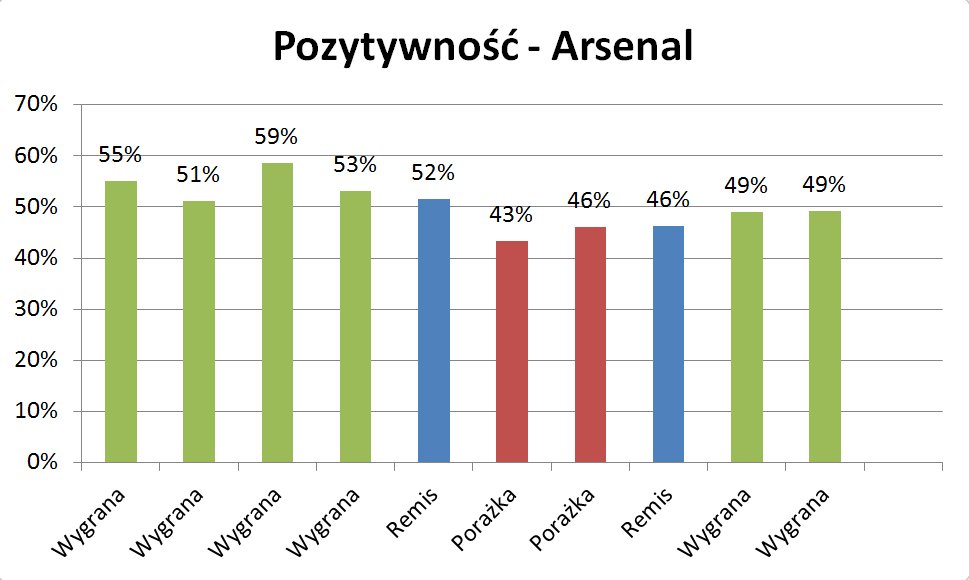
\includegraphics[width=100mm]{img/pozytywnosc-arsenal.png}
\caption{Wyniki spotkań Arsenalu a sentyment wpisów}
\label{image:pozytywnosc-arsenal}
\end{figure}


\begin{figure}[ht!]
\centering
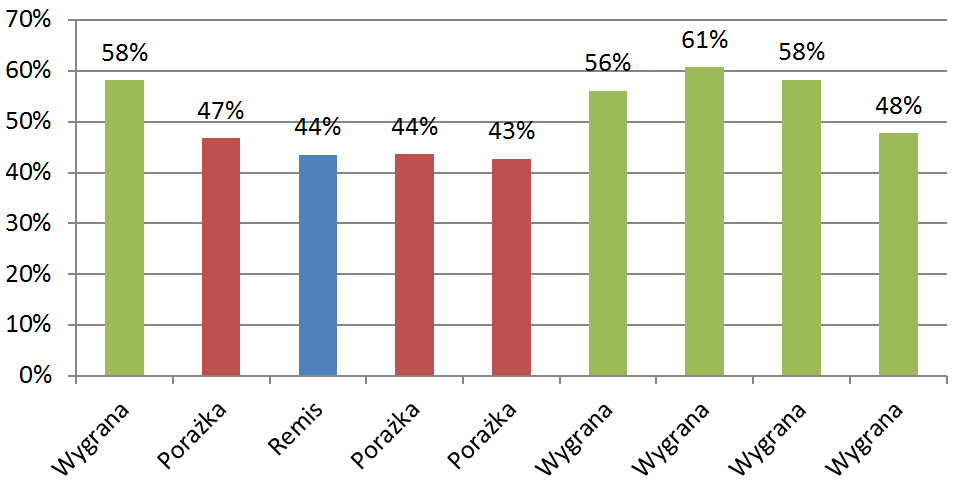
\includegraphics[width=100mm]{img/pozytywnosc-munited.png}
\caption{Wyniki spotkań Manchesteru United a sentyment wpisów}
\label{image:pozytywnosc-munited}
\end{figure}

Jak widać na załączonych powyżej wykresach nasłuchując wpisów ze słowami kluczowymi
z poszczególnych drużyn, sentyment prezentowany przez kibiców jest dokładnie taki
sam jak wynik meczu. 


\clearpage
\subsection{Liczba i rodzaje komunikacji między zwolennikami i przeciwnikami klubów}
% retweety pozytywne zwolennicy, replies negatywne
% przeciwnicy, itd

Przeciwnicy najczęściej dyskutują z przeciwnikami \ref{image:replies-munited}

\begin{figure}[ht!]
\centering
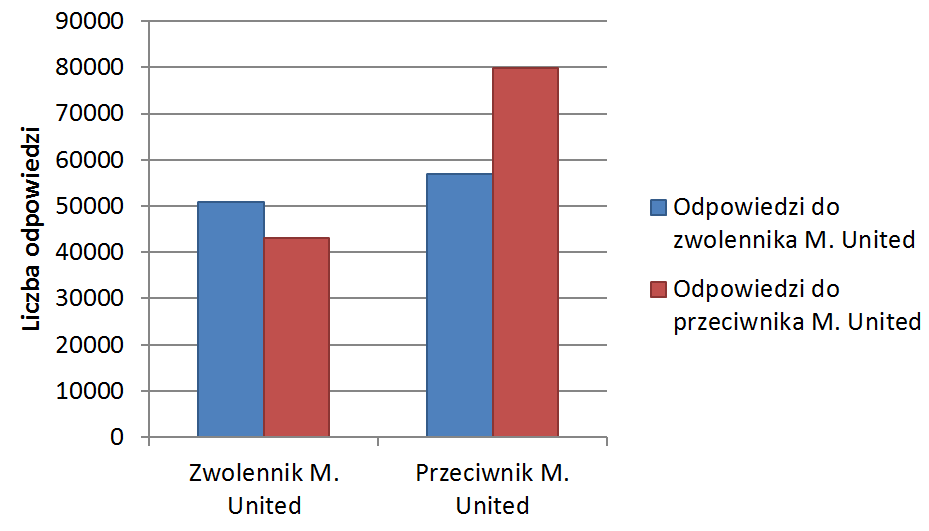
\includegraphics[width=120mm]{img/replies-munited.png}
\caption{Charakterystyka odpowiedzi wśród wpisów dotyczących Manchesteru United}
\label{image:replies-munited}
\end{figure}

Zwolennicy najczęściej retweetują wpisy zwolenników \ref{image:retweety-munited}

\begin{figure}[ht!]
\centering
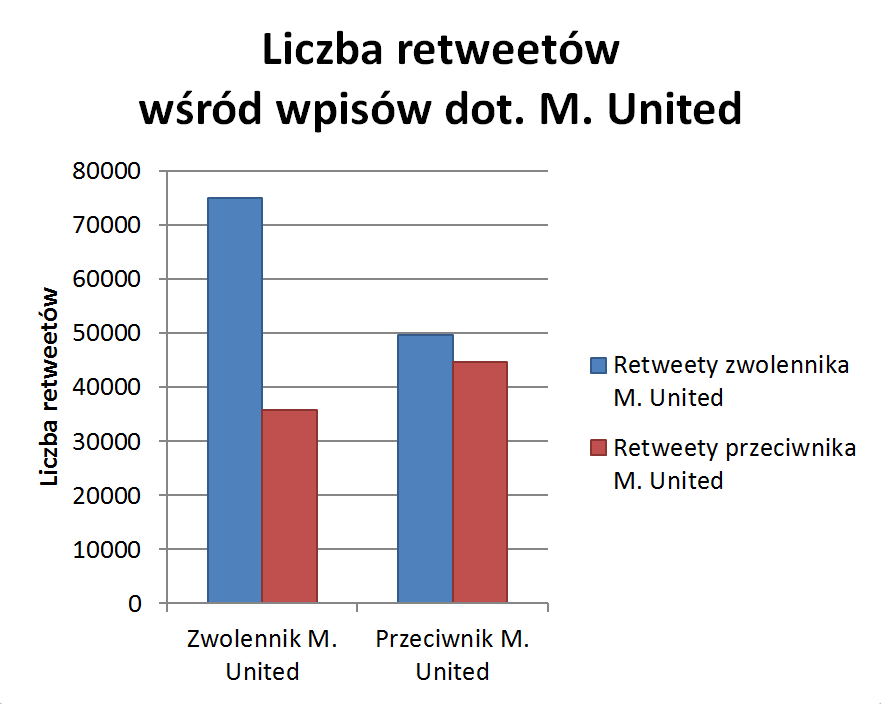
\includegraphics[width=120mm]{img/retweety-munited.png}
\caption{Charakterystyka retweetów wśród wpisów dotyczących Manchesteru United}
\label{image:retweety-munited}
\end{figure}


\subsection{Sentyment odpowiedzi między zwolennikami i przeciwnikami drużyny}

\subsubsection{Gdy odpowiada zwolennik Arsenalu}

Zwolennicy bardzo często odpowiadają innym zwolennikom na wpisy pozytywne,
również wpisami pozytywnymi \ref{image:reply-sentiment-zwolennik-zwolennik}.
\begin{figure}[ht!]
\centering
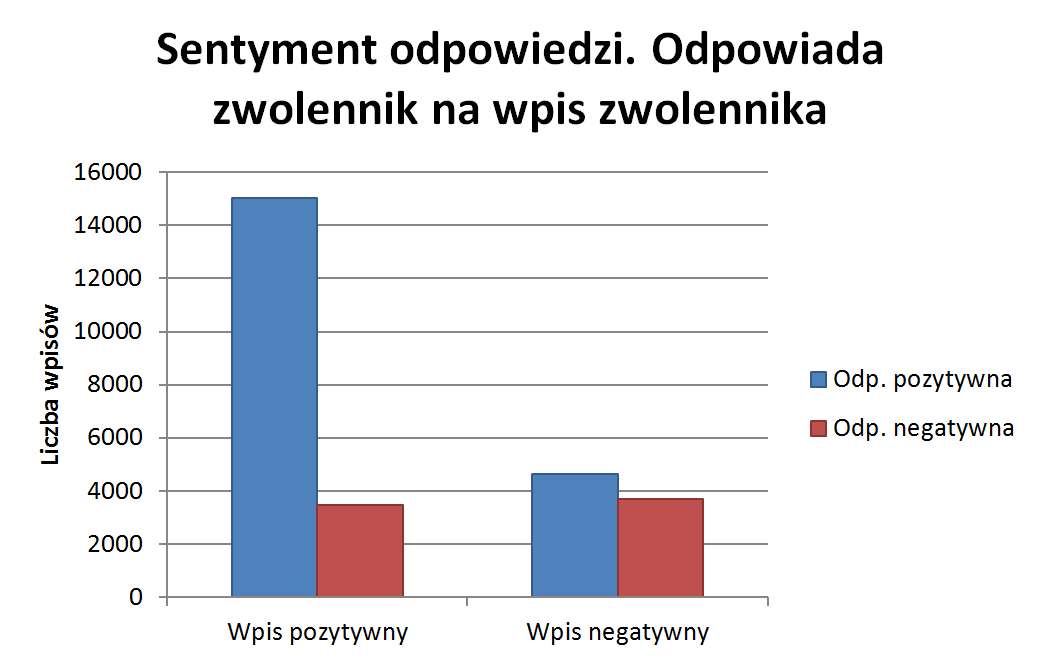
\includegraphics[width=120mm]{img/reply-sentiment-zwolennik-zwolennik.png}
\caption{Sentyment odpowiedzi}
\label{image:reply-sentiment-zwolennik-zwolennik}
\end{figure}

Zwolennicy nawet na wpisy negatywne starają się odpowiadać pozytywnie
 \ref{image:reply-sentiment-zwolennik-przeciwnik}.
 
\begin{figure}[ht!]
\centering
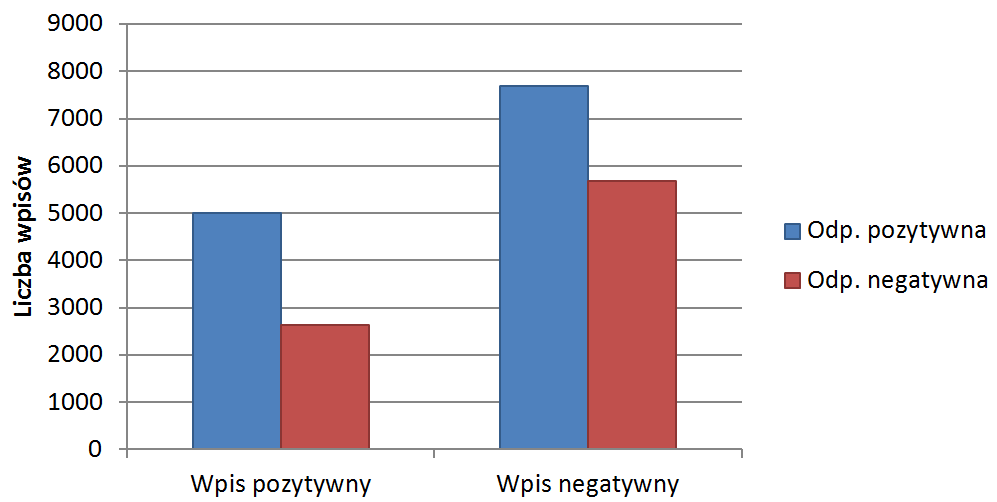
\includegraphics[width=120mm]{img/reply-sentiment-zwolennik-przeciwnik.png}
\caption{Sentyment odpowiedzi}
\label{image:reply-sentiment-zwolennik-przeciwnik}
\end{figure}


\clearpage
\subsubsection{Gdy odpowiada przeciwnik Arsenalu}

Przeciwnicy odpowiadają negatywnie zwolennikom zarówno na wpisy pozytywne jak 
i negatywne \ref{image:reply-sentiment-przeciwnik-zwolennik}.

\begin{figure}[ht!] \centering
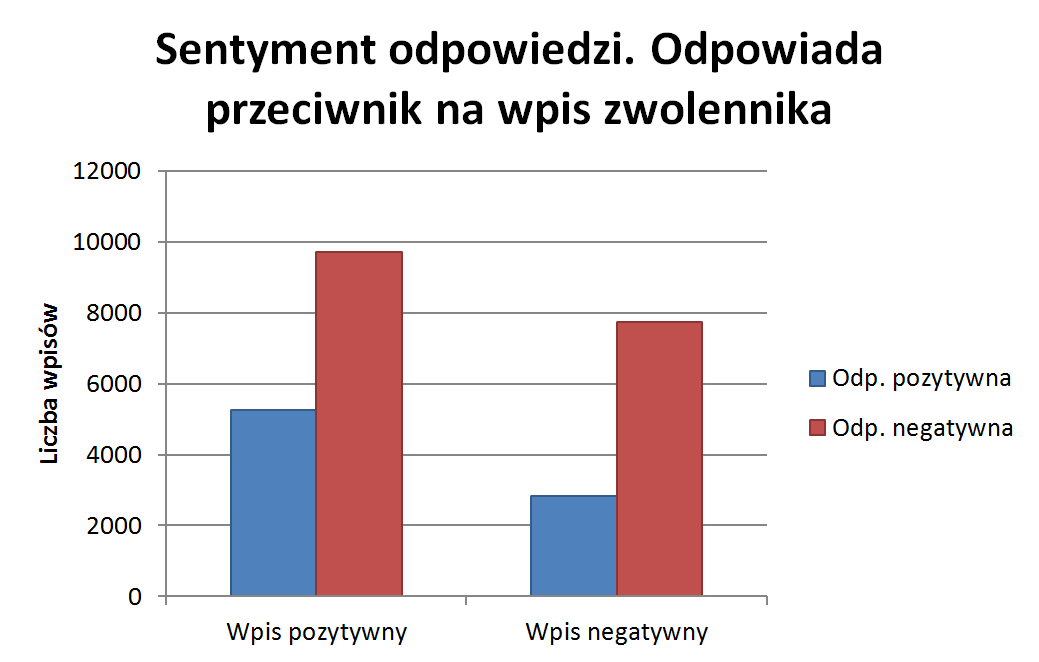
\includegraphics[width=120mm]{img/reply-sentiment-przeciwnik-zwolennik.png}
\caption{Sentyment odpowiedzi}
\label{image:reply-sentiment-przeciwnik-zwolennik}
\end{figure}


Przeciwnicy klubu najchętniej odpowiadają innym przeciwnikom na wpisy negatywne
wpisami negatywnymi \ref{image:reply-sentiment-przeciwnik-przeciwnik}.

\begin{figure}[ht!] \centering
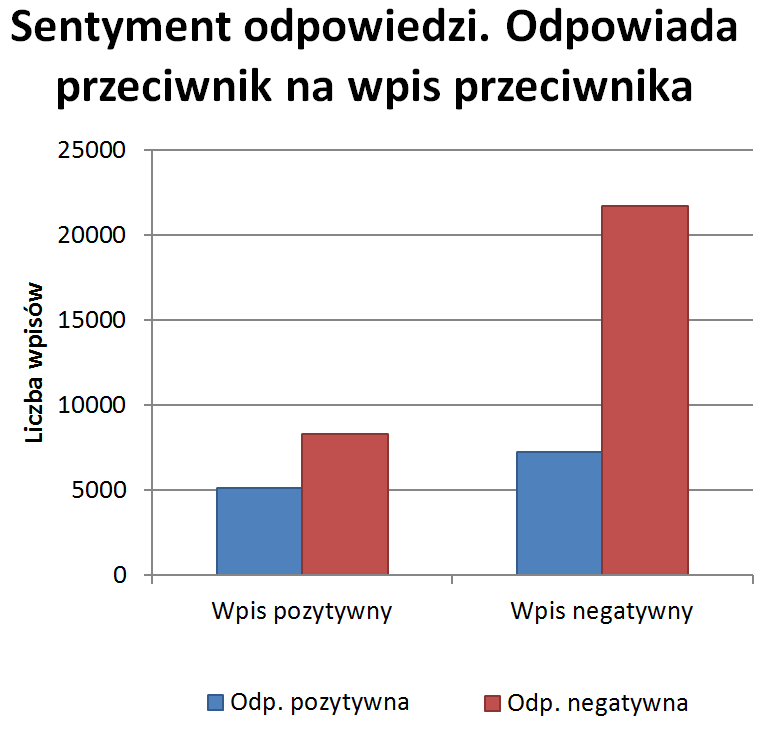
\includegraphics[width=120mm]{img/reply-sentiment-przeciwnik-przeciwnik.png}
\caption{Sentyment odpowiedzi}
\label{image:reply-sentiment-przeciwnik-przeciwnik}
\end{figure}










%%%%%%%%%%%%%%%%%%%%%%%%%%%%%%%%%%%%%%%%%%%%%%%%%%%%%%%%%% ANALIZA GEOGRAFICZNA
\clearpage
\section{Analiza geograficzna}
\label{section:analizageograficzna}
%Odległość użytkowników komunikujących się ze sobą od siebie

Im kibice są fizycznie bliżej siebie, tym częściej się ze sobą komunikują, 
co przedstawia poniższy wykres \ref{image:relacje-a-odleglosc}.
Wartości odległości w kolejnych kolumnach rosną wykładniczo,
a liczba użytkowników, między którymi doszło do wymiany wiadomości
pozostaje na takim samym rzędzie wielkości. Między użytkownikami oddalonymi
od siebie o maksymalnie 10 km doszło do tylu samo wymian wiadomości,
jak między użytkownikami oddalonymi od 10 do 100 km, czy między użytkownikami
oddalonymi od 100 do 1000 km od siebie.

\begin{figure}[ht!]
\centering
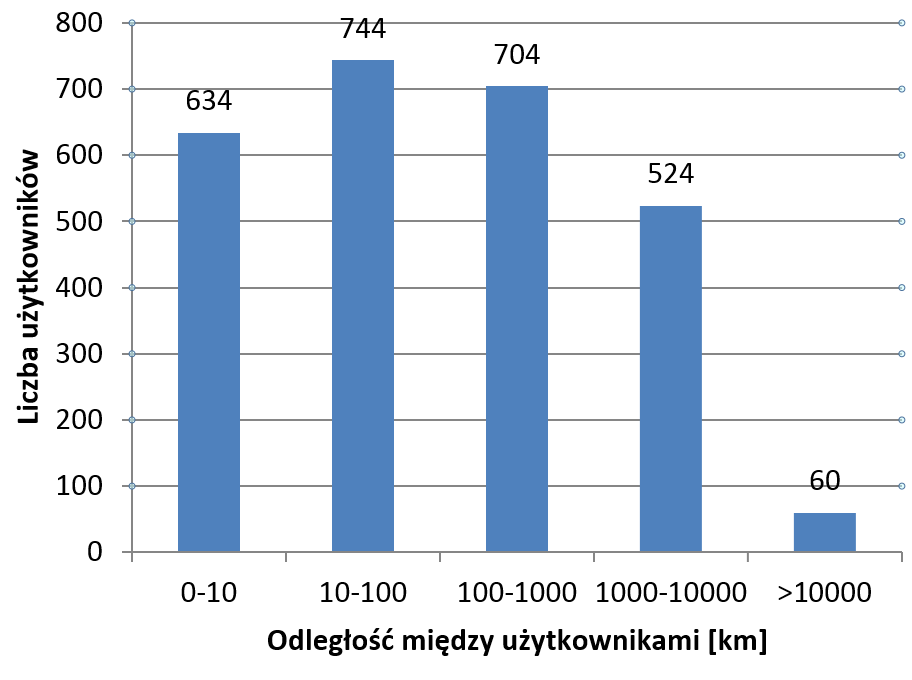
\includegraphics[width=120mm]{img/relacje-a-odleglosc.png}
\caption{Relacje między użytkownikami a odległość fizyczna między nimi}
\label{image:relacje-a-odleglosc}
\end{figure}

%Odległość od stadionu zwolenników, przeciwników 
%Odległość od stadionu a sentyment
%Miejscowości a sentyment 
%Kraje, a sentyment








%%%%%%%%%%%%%%%%%%%%%%%%%%%%%%%%%%%%%%%%%%%%%%%%%%%%%%%%%%%%%%%%%% ANALIZA GRUP
\clearpage
\section{Analiza grup}
\label{section:analizagrup}
Podobieństwo w meczach Arsenalu \ref{image:grupy-arsenal}
 
\begin{figure}[ht!]
\centering
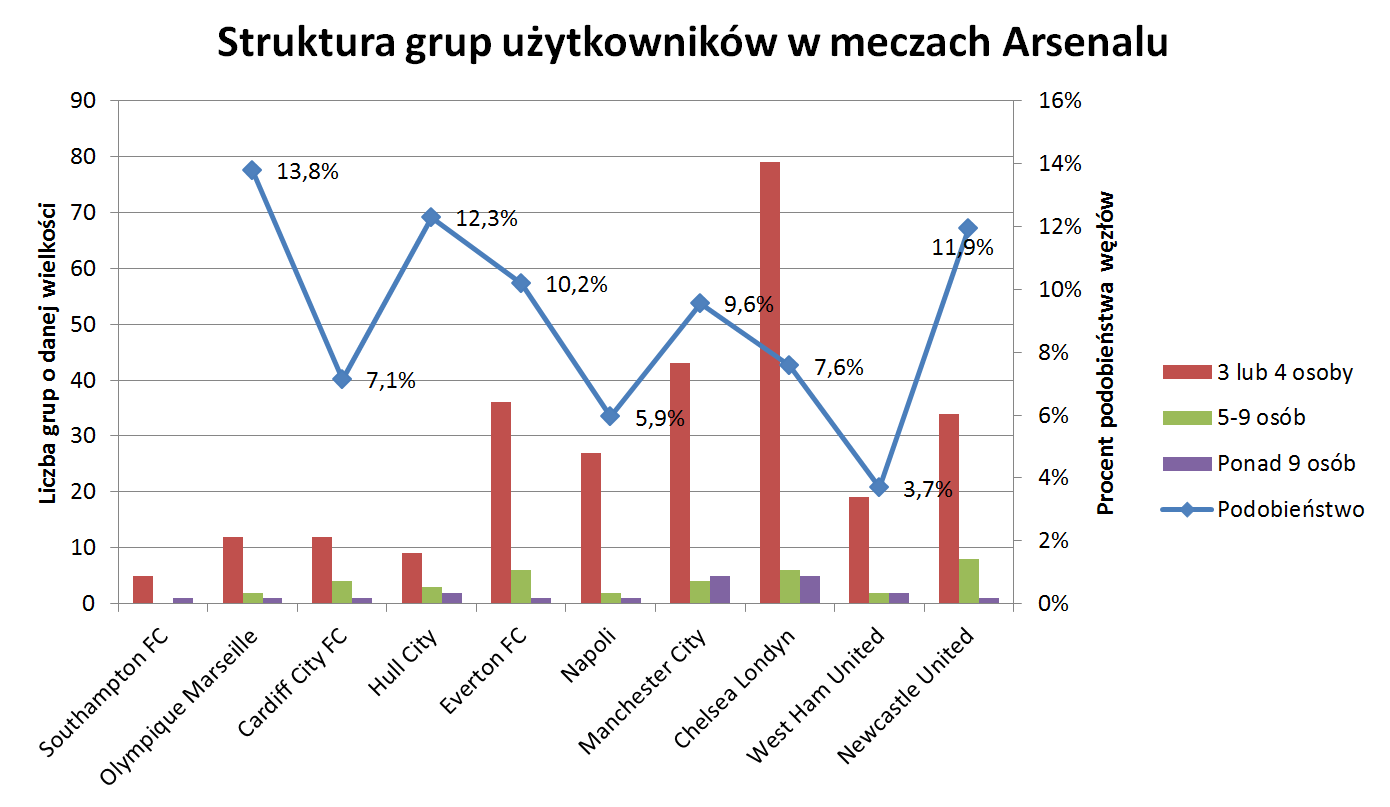
\includegraphics[width=120mm]{img/grupy-arsenal.png}
\caption{Struktura grup użytkowników w meczach Arsenalu}
\label{image:grupy-arsenal}
\end{figure}

Podobieństwo w meczach Manchesteru United \ref{image:grupy-munited}

\begin{figure}[ht!]
\centering
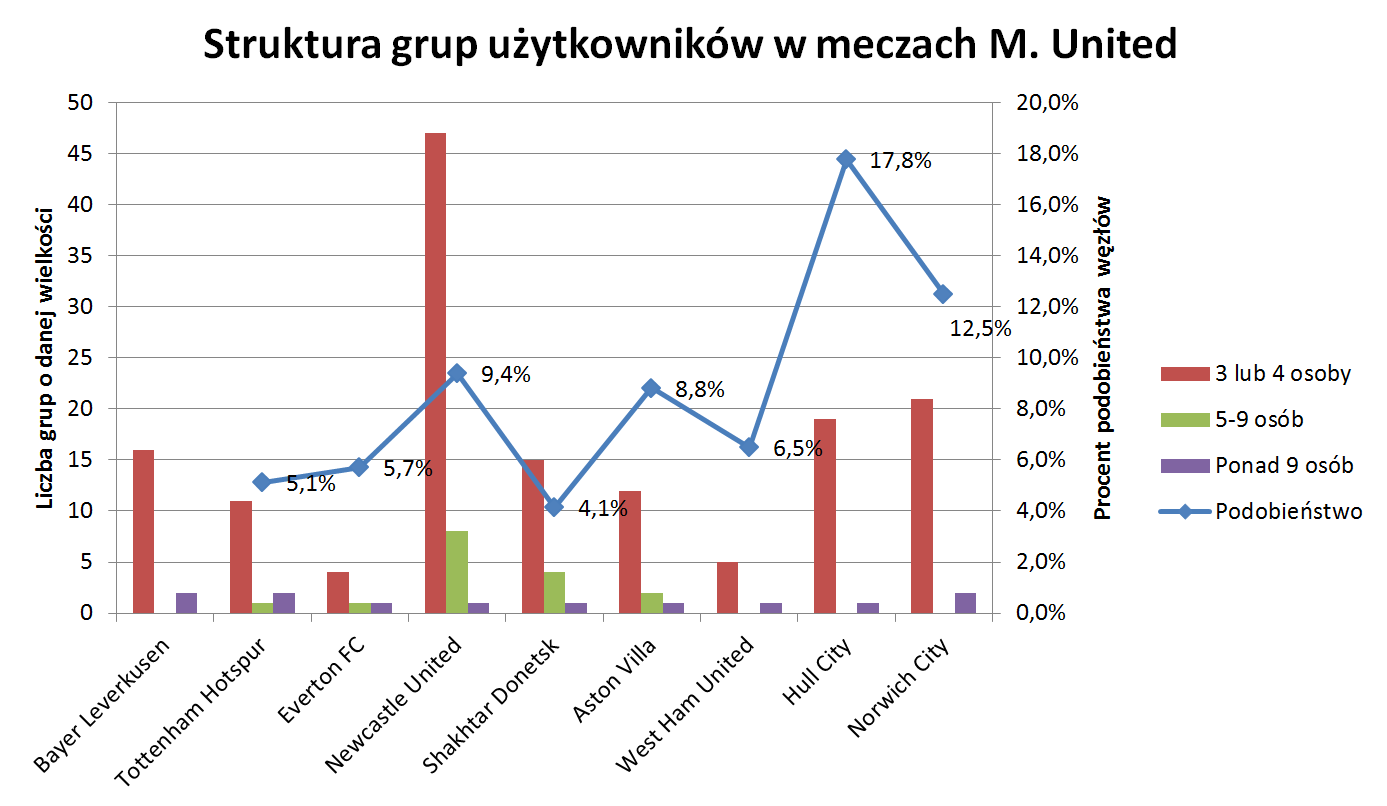
\includegraphics[width=120mm]{img/grupy-munited.png}
\caption{Struktura grup użytkowników w meczach Manchesteru United}
\label{image:grupy-munited}
\end{figure}

% Podobieństwo węzłów między meczami 
% Podobieństwo grafów między meczami 
% Między mało popularnymi spotkaniami wysoki stopień podobieństwa
% +Sentyment a wielkość grupy

